% !TEX root =/main.tex
\chapter{Processes}

We want to be able to run several programs at the same time, but our cpu is only able to run one program at the time. This way of looking at the problem is impossible to solve. What we actually want is the feeling of several programs running at the same time, and while a cpu core cannot execute several programs at once, it can continually switch between executing several different processes without completing them. This is called content switching.

Think of the cpu as a human performing a task, if we for example are cooking and while cutting the vegetables we accidentally cut ourselves, we don't need to finish cooking before rinsing and plastering the wound, we instead stop cooking for a while to fix the higher priority task; stopping the bleeding, before continuing to cook.

\section{Introduction to processes}

A process is an execution of a program, the execution must be sequential.
The program is the executable entity on disk, a process is when it runs, active.
When the executable program is loaded into memory, it becomes a process.
When a program is run several times, simultaneously or at different time, they are separate processes and cannot affect each others.
A process can have sub processes.

\begin{minipage}{.3\textwidth}
	\begin{figure}[H]
		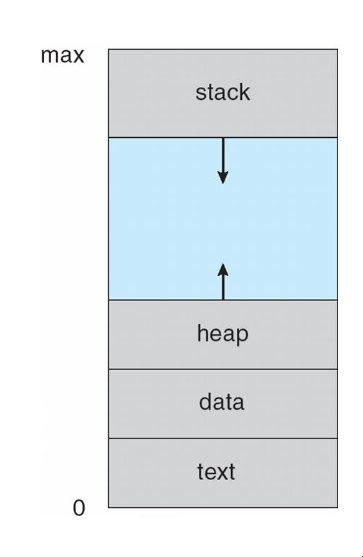
\includegraphics[width=\textwidth]{images/process_in_mem.png}
		\label{fig:proc_in_mem}
		\caption{How a process' memory is allocated}
	\end{figure}

\end{minipage}\begin{minipage}{0.65\textwidth}
	\begin{description}
		\item[Text section]  The program code.
		\item[Data section] Data section containing global variables.
		\item[Heap section] Heap containing memory dynamically allocated during run time.
		\item[Stack section] Stack containing temporary data like f parameters, return addresses, local variables.
	\end{description}
\end{minipage}

\begin{figure}[H]
	\centering
	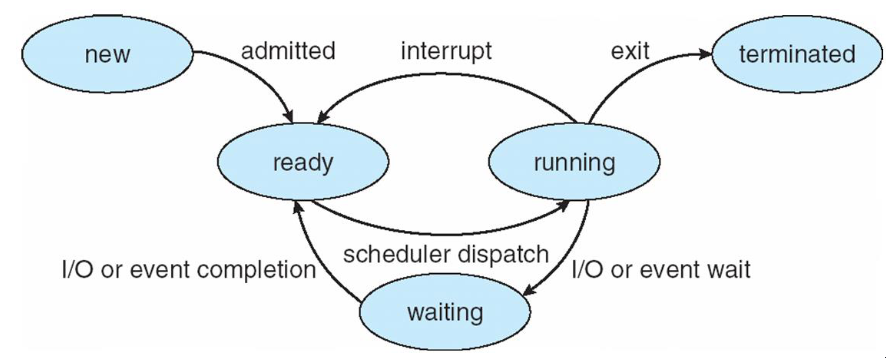
\includegraphics[width=0.8\textwidth]{images/diagram_process_state.png}
	\label{fig:proc_state_diagram}
	\caption{Diagram of process state}
\end{figure}

\subsection{Context switching}
To be able to switch between executing several different processes, a concept called PCB (Process Control Block) is utilized.

\begin{minipage}{.3\textwidth}
	\begin{figure}[H]
		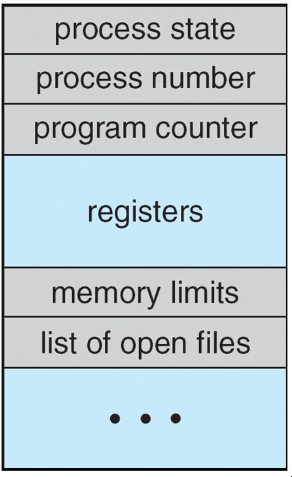
\includegraphics[width=\textwidth]{images/pcb.png}
		\label{fig:pcb}
		\caption{A process content block}
	\end{figure}

\end{minipage}\begin{minipage}{0.65\textwidth}
	\begin{description}
		\item[Process state]							running, waiting, etc.
		\item[Program counter]						location of next instruction to execute
		\item[CPU registers]							contents of all process-centric registers
		\item[CPU scheduling information]		priorities, scheduling queue pointers
		\item[Memory-management ]					memory allocated to the process
		\item[Accounting information]				CPU used, clock time elapsed since start, time limits
		\item[I/O status information]				I/O devices allocated to process, list of open files
	\end{description}
\end{minipage}

\section{Process scheduling}

How we schedule which process should be executed next is a very important task, since a lot of processes are usually waiting for data from devices, it can be very time inefficient to store all processes in a list and just executing the first  ready process. To speed up the execution we instead separate processes into different lists, when a process is waiting for input from a certain I/O device, we put it in a list connected to that I/O device, and when a process is waiting for the disk, we put it into a list connected to the disk, this way we limit the numbers of processes we need to check when choosing which process should be the next to run.

\begin{figure}[H]
	\centering
	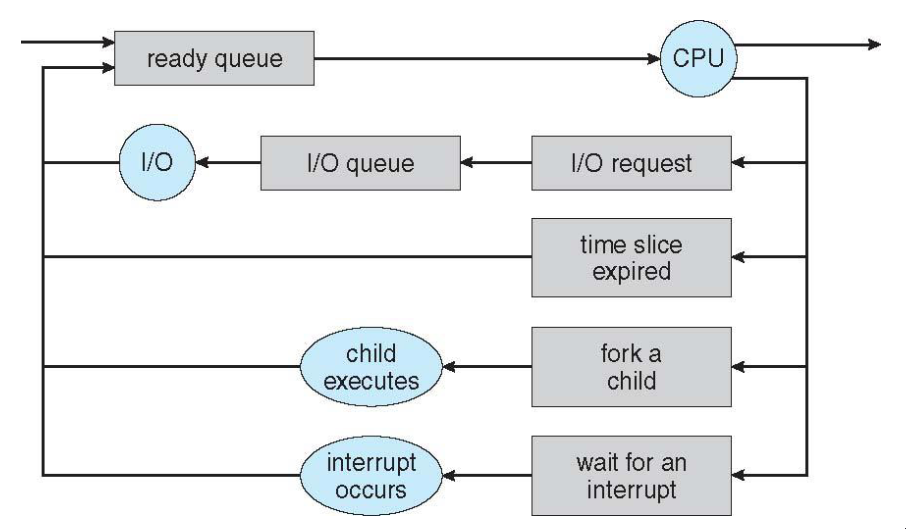
\includegraphics[width=.5\textwidth]{images/scheduling_process.png}
	\label{fig:process_scheduling}
	\caption{Example of how we choose next process to run}
\end{figure}
\section{Operations on processes}
\subsection{Process creation}
The user needs to be provided the ability to create and terminate processes. Since processes can't be created from nowhere, we have a higher process which can create child processes, to be able to do this, we need a system call to create processes.

From this we get a tree structure of processes, with the root process, init, always at the top, with pid = 1.

The command we use to be able to create new processes is fork(), which creates a copy of the current process, if we then want that new process to do something different than the parent program, we have a command exec(), which helps us load a new program into the process. NOTE: When calling fork(), the child and the parent will get differing results, provided nothing went wrong, the child process will get the value 0 returned while the parent gets the process ID of the created child returned.
\begin{figure}[H]
	\centering
	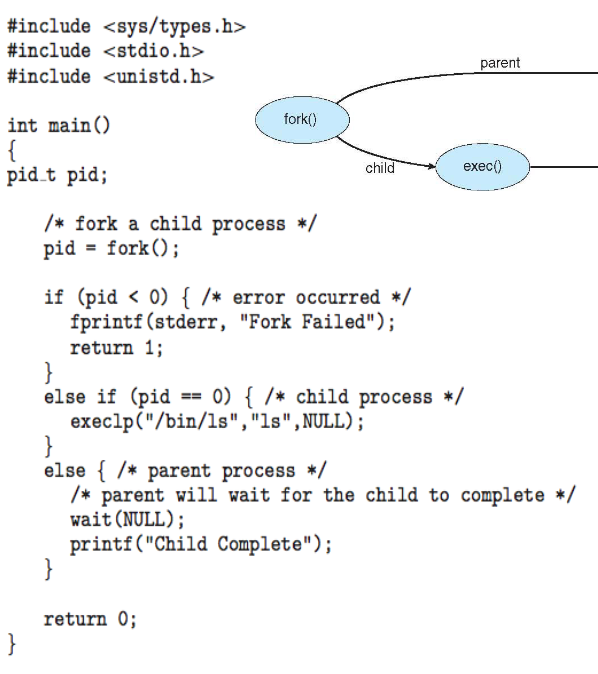
\includegraphics[width=.6\textwidth]{images/fork.png}
	\label{fig:fork}
	\caption{A C program creating a child}
\end{figure}

\subsection{Process termination}

When a process is finished executing, it calls the operating system using exit(), this tells the operating system to clean up after the program, free allocated memory and stuff.

Sometimes the termination of a process cannot be completed, for example if the child process is done, trying to return its result to the parent \textbf{but} the parent hasn't waited for the response, the process cannot be completely removed.



\section{Interprocess communication}
